\documentclass[../bericht.tex]{subfiles}

\begin{document}

  \chapter{Einleitung}

    Die Sekunde ist das $9.192.631.770$-fache der Periodendauer der dem \"Ubergang zwischen den beiden Hyperfeinstrukturniveaus des Grundzustandes von Atomen des Nuklids $\mathrm{^{133}Cs}$ entsprechenden Strahlung - so die Definition nach dem SI-Einheitensystem. Genau diese Periodendauer soll im folgenden Versuch gemessen werden. Hierzu werden sowohl die Feinstruktur als auch die Hyperfeinstruktur erkl\"art und mittels der dopplerfreien Spektroskopie der \"Ubergang aufgel\"ost.


  \chapter{Versuch}

    \section{Feinstruktur}
    \label{sec:feinstruktur}

      Nach dem semiklassischen Atommodell kreisen die negativ geladenen Elektronen auf einer Kreisbahn um den positiv geladenen Atomkern. Die Rotation stellt einen Kreisstrom dar. Dieser erzeugt ein magnetisches Dipolmoment, welches \"uber den Bahndrehimpuls $\vec{l}$ ausgedr\"uckt werden kann. Gem\"a\ss dem Stern-Gerlach-Experiment (und anderen Experimenten) haben Elektronen ein weiteres magnetisches Dipolmoment inne, welchem der Spin $\vec{s}$ zugrunde liegt. Die beiden magnetischen Momente wechselwirken in der sogenannten \textit{Spin-Bahn-Kopplung}. Je nach Einstellung des Elektronenspins (\textit{Spin-up}/ \textit{Spin-down}, d.h. f\"ur die $z$-Komponente des Spins $s_z=\pm \frac{\hslash}{2}$) ergibt sich eine positive, bzw. negative Energiekorrektur $\Delta E_{l,s}$, die sogenannte \textit{Spin-Bahn-Kopplungsenergie}.

      Bei der mathematischen Betrachtung sind f\"ur die \textit{Feinstrukturaufspaltung} au\ss{}erdem relativistische Effekte zu beachten. Auf der Umlaufbahn um den ruhenden Kern dreht sich das Elektron einmal um die zum Drehimpuls parallele Achse. Dies f\"uhrt zu einer Korrektur der kinetischen Energie $\Delta E_\mathrm{rel}$.

      Zuletzt muss der \textit{Darwin-Term} $\Delta E_\mathrm{Darwin}$ ber\"ucksichtigt werden. Als Folge der relativistischen Zitterbewegung des Elektrons auf seiner Kreisbahn verkompliziert sich die elektrostatische Wechselwirkung zwischen Elektron und Atomkern.
      \medskip

      Die gesamte Energiekorrektur
      \begin{equation*}
        \Delta E = \Delta E_{l,s} + \Delta E_\mathrm{rel} + \Delta E_\mathrm{Darwin}
      \end{equation*}
      f\"uhrt zur sogenannten \textit{Feinstrukturaufspaltung}.
      \medskip

      Zur Beschreibung dieser Zust\"ande wird der Gesamtdrehimpuls $\vec{j}=\vec{l}+\vec{s}$ mit der zugeh\"origen gutartigen Gesamtdrehimpulsquantenzahl $j$ eingef\"uhrt. Letzte kann die Werte
      \begin{equation*}
        j=+\frac{1}{2} \quad\text{f\"ur}\quad l=0
      \end{equation*}
      und
      \begin{equation*}
        j=l\pm \frac{1}{2}\quad\text{f\"ur}\quad l>0
      \end{equation*}
      annehmen. Somit spalten alle Zust\"ande mit $l>0$ in zwei \textit{Feinstrukturniveaus} auf.


    \section{Hyperfeinstruktur}
    \label{sec:hyperfeinstruktur}

      Analog zum Spin des Elektrons wird auch dem r\"aumlich ausgedehnten Atomkern ein Spin zugeordnet, der sogenannte \textit{Kernspin} $\vec{I}$. Das dem Spin zugeordnete magnetische Moment des Kerns wechselwirkt mit dem Gesamtspin des Elektrons $\vec{j}$. Wiederum kommt es je nach Ausrichtung des Kernspins zu einer Energiekorrektur welche positiv und negativ ausfallen kann. Die Projektion auf die $z$-Richtung von $\vec{I}$ kann die $(2I + 1)$ Werte
      \begin{equation*}
        I_z=m_I \cdot \hslash\quad\text{mit}\quad -I\le m_I \le +I
      \end{equation*}
      annehmen. Zur Zustandsbeschreibung wird nun der Gesamtdrehimpuls des Atoms $\vec{F}=\vec{j}+\vec{I}$ mit der zugeh\"origen gutartigen Quantenzahl $F$,
      \begin{equation*}
        |j-I| \le F\le |j + I|
      \end{equation*}
      eingef\"uhrt. Die \textit{Feinstrukturniveaus} spalten also in
      \begin{equation*}
        \begin{cases}
            (2I+1), & I<j\\
            (2j+1), & j<I
        \end{cases}
      \end{equation*}
      \textit{Hyperfeinstrukturniveaus} auf. Aufgrund der im Vergleich zum Elektron extrem gro\ss{}en Masse des Kerns
      \begin{equation*}
        m_\mathrm{Kern}\approx Z\cdot 1836 \cdot m_\mathrm{e},
      \end{equation*}
      mit der Kernladungszahl $Z$, ist die Energieaufspaltung in Folge der \textit{Hyperfeinstruktur} sehr klein. Um diese zu messen ist also extrem schmalbandiges Licht notwendig, welches gleichzeitig so intensiv sein muss, dass ein messbares Signal entsteht. Weil Monochromatoren zu breitbandig sind, erfordert das Experiment also einen Laser.


    \section{Termschema von C\"asium}
    \label{sec:termschema-caesium}

      Im Versuch wird das Nuklid $\mathrm{^{133}Cs}$ verwendet. F\"ur die Zust\"ande wird die Nomenklatur $n^{2s+1}l_j$  verwendet. Der relevante Teil des Termschemas von C\"asium f\"ur den Versuch, d.h. der Grundzustand $\mathrm{6^2 S_{1/2}}$ und der angeregte Zustand $\mathrm{6^2P_{3/2}}$ mit Feinstrukturaufspaltung und Hyperfeinstrukturaufspaltung sind in \cref{fig:feinstruktur-hyperfeinstruktur} abgebildet. Die Kernspinquantenzahl ist $I=\frac{7}{2}$. Weiter sind die erlaubten angeregten optischen \"Uberg\"ange rot eingezeichnet. F\"ur diese ist zu beachten, dass anregende Photonen einen Spin von $1$ tragen. Bei Verwendung von linear polarisiertem Licht gelten die \"Ubergangsregeln
      \begin{equation*}
        \Delta l = 1\quad \text{und}\quad \Delta F = -1,0,+1.
      \end{equation*}

      \begin{figure}[tb]
        \centering
        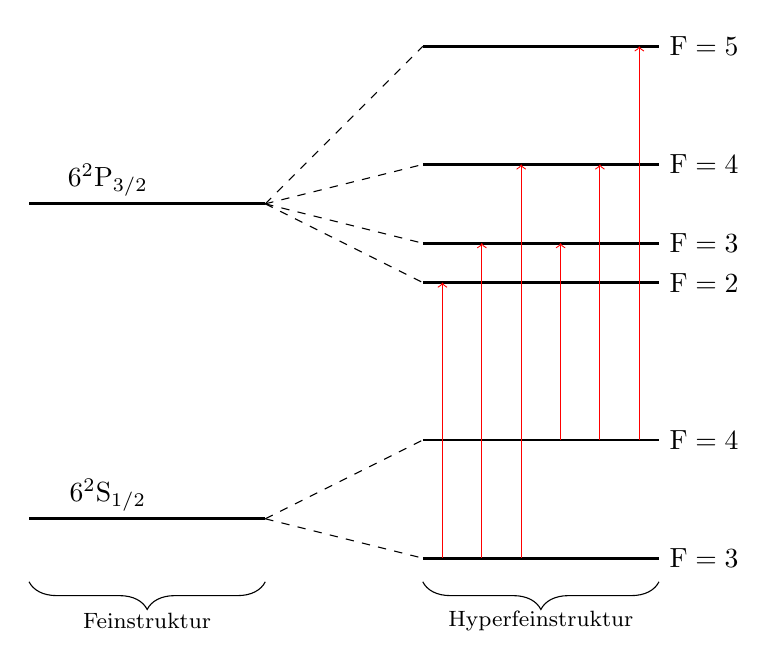
\begin{tikzpicture}
          % angeregte Niveaus
          \node at (1,4.3) {$\mathrm{6^2P_{3/2}}$};
          \draw[line width=1pt] (0,4)--(3,4);
          \draw[line width=1pt] (5,6)--(8,6) node[anchor=west] {$\mathrm{F=5}$};
          \draw[line width=1pt] (5,4.5)--(8,4.5) node[anchor=west] {$\mathrm{F=4}$};
          \draw[line width=1pt] (5,3.5)--(8,3.5) node[anchor=west] {$\mathrm{F=3}$};
          \draw[line width=1pt] (5,3)--(8,3) node[anchor=west] {$\mathrm{F=2}$};
          \draw[dashed] (3,4)--(5,6);
          \draw[dashed] (3,4)--(5,4.5);
          \draw[dashed] (3,4)--(5,3.5);
          \draw[dashed] (3,4)--(5,3);
          % Grundzustand Niveaus
          \node at (1,0.3) {$\mathrm{6^2S_{1/2}}$};
          \draw[line width=1pt](0,0)--(3,0);
          \draw[line width=1pt] (5,1)--(8,1) node[anchor=west] {$\mathrm{F=4}$};
          \draw[line width=1pt] (5,-0.5)--(8,-0.5) node[anchor=west] {$\mathrm{F=3}$};
          \draw[dashed] (3,0)--(5,1);
          \draw[dashed] (3,0)--(5,-0.5);
          % \"Uberg\"ange
          % Unterer Grundzustand
          \draw[color=red, ->] (5.25,-0.5)--(5.25,3);
          \draw[color=red, ->] (5.75,-0.5)--(5.75,3.5);
          \draw[color=red, ->] (6.25,-0.5)--(6.25,4.5);
          % Oberer Grundzustand
          \draw[color=red, ->] (6.75,1)--(6.75,3.5);
          \draw[color=red, ->] (7.25,1)--(7.25,4.5);
          \draw[color=red, ->] (7.75,1)--(7.75,6);
          % Fein- und Hyperfeinstruktur
          \draw [decorate,decoration={brace,mirror,amplitude=10pt}] (0,-0.8) -- (3,-0.8) node [black,midway,yshift=-14pt] {\footnotesize Feinstruktur};
          \draw [decorate,decoration={brace,mirror,amplitude=10pt}] (5,-0.8) -- (8,-0.8) node [black,midway,yshift=-14pt] {\footnotesize Hyperfeinstruktur};
        \end{tikzpicture}
        \caption{Termschema von $\mathrm{^{133}Cs}$ ($I=\frac{7}{2}$) mit Feinstruktur und Hyperfeinstruktur. Die erlaubten Anregungs\"uberg\"ange sind rot markiert. }
        \label{fig:feinstruktur-hyperfeinstruktur}
      \end{figure}


    \section{Diodenlaser}
    \label{sec:diodenlaser}

      Es folgt eine Kurzfassung von ??? zur Funktion von Diodenlasern.

      Diodenlaser sind aus Halbleitern aufgebaut. Bei der Rekombination von Elektronen im Leitungsband mit den L\"ochern im Valenzband wird das Laserlicht emittiert. Der Hauptteil eines Diodenlasers besteht aus einem $p-n$-\"Ubergang, welcher durch Dotierung erzeugt wird. Die Besetzungsinversion mit L\"ochern im Valenzband und Elektronen im Leitungsband wird durch das Anlegen einer Spannung erreicht. Dieser Prozess ist der Pumpprozess des Lasers. Die Rekombination der L\"ocher und Elektronen kann spontan oder stimuliert erfolgen. Das dabei emittierte Licht ist nur koh\"arent, falls die stimulierte Emission \"uberwiegt. Aufgrund des hohen Brechungsindexes $n$ der Halbleiterkristalle betr\"agt die Reflektivit\"at der Grenzfl\"ache zu Vakuum in etwa $\SI{30}{\percent}$. Damit k\"onnen die Kristalle selbst, ohne weitere Behandlung, als Resonatoren fungieren. Diejenige Seite, auf der kein Licht austreten soll, wird zus\"atzlich verspiegelt. F\"ur die Ausbildung von stehenden Wellen im Resonator gilt der Zusammenhang
      \begin{equation*}
        \lambda = \frac{2nL}{m}.
      \end{equation*}
      Hierbei ist $\lambda$ die Wellenl\"ange des Lichts, $L$ die L\"ange des Resonators (Halbleiterkristalls) und $m$ eine nat\"urliche Zahl.

      Einer der Vorteile eines Diodenlasers ist dessen Durchstimmbarkeit bez\"uglich der Frequenzen. In Abh\"angigkeit der Betriebstemperatur $T$ und der Stromst\"arke $I$ \"andert sich die Frequenz der Laserstrahlung. Die Temperatur beeinflusst die Ausdehnung des Kristalls und damit die L\"ange des Resonators. Unter Voraussetzung einer konstanten Temperatur \"andert sich mit der Stromst\"arke die Ladungstr\"agerdichte im Halbleiter. Damit \"andert sich auch der Brechungsindex des Kristalls und somit die optische L\"ange des Resonators.
      Die Durchstimmbarkeit ist f\"ur diesen Versuch von Bedeutung, um die Resonanzfrequenz von C\"asium zu treffen.
      \medskip

      Weiter weist ein Diodenlaser, wie alle Laser, eine schmale Linienbreite auf. Dieser Vorteil, welcher f\"ur dieses Experiment von großer Bedeutung ist, wird in \cref{sec:linienbreite} vertieft.


      \subsection{Laserschwelle des verwendeten Diodenlasers}
      \label{subsec:laserschwelle}

        Der in diesem Versuch verwendete Diodenlaser weist den in \cref{fig:laserschwelle} abgebildeten Zusammenhang zwischen Eingansstrom und Ausgangsleistung auf. Die lineare Regression f\"ur Messpunkte mit Eingangsstrom $I\ge 31$ liefert die Gerade
        \begin{equation}
          P(I)=-\SI{5,21(6)}{\milli\watt} + \SI{0,156(1)}{\volt}\cdot I
          \label{eq:laserschwellen-plot}
        \end{equation}
        Und damit die Laserschwelle
        \begin{equation}
          I_\mathrm{Schwelle}=\SI{33,37(56)}{\ampere}.
          \label{eq:laserschwelle}
        \end{equation}
        Gemessen wurde die Ausgangsleistung in Abh\"angigkeit des \textit{Coarse} der Spannungsquelle. Mithilfe von \textit{Coarse}-Stromst\"arke-Kennlinie des Netzteils des Diodenlasers (\cref{sec:netzteil-kennlinie}) wird die Eingangsstromst\"arke des Lasers ermittelt. Diese Daten liegen nicht in digitaler Form vor und mussten deshalb vom Graphen abgelesen werden. Hierbei ist ein nicht zu vernachl\"assigender Fehler aufgetreten, der, zusammen mit dem unbekannten Fehler der des Graphen selber, auf
        \begin{equation*}
          \delta I = \pm \SI{2}{\milli\ampere}
        \end{equation*}
        gesch\"atzt wird. Zudem liegt der Fehler des Powermeters??? bei
        \begin{equation*}
          \delta P = 0,003 \cdot P.
        \end{equation*}
        Beide Fehler sind mithilfe der Fehlerbalken in \cref{fig:laserschwelle} angegeben. Bei der Berechnung der linearen Regression wurde der Fehler des Powermeters mit einer $\frac{1}{\mathrm{Fehler}}$-Gewichtung ber\"ucksichtigt. Die Messungen wurden bei der Diodenlasertemperatur
        \begin{equation*}
          T=\SI{21,4(20)}{\celsius}
        \end{equation*}
        durchgef\"uhrt. W\"ahrend die Anzeige des Regelungsinstruments den Wert laut technischer Daten pr\"aziser angibt, ist das Ger\"at seit Jahren nicht geeicht geworden. Deshalb dient die Anzeige nur als Anhaltspunkt, bzw. f\"ur Temperaturdifferenzen, jedoch nicht f\"ur absolute Temperaturmessungen. Dementsprechen gro\ss{} ist der Fehler mit $\SI{2}{\celsius}$  gew\"ahlt.

        \begin{figure}[tb]
          \centering
          \begin{tikzpicture}
              \def\Imin{0}
      				\def\Imax{100}
      				\def\Pmin{0}
      				\def\Pmax{10}eq:laserschwelle
              %
              \begin{axis}[
                /tikz/line join=bevel,
                width=0.8*\textwidth,
                height=0.5*\textwidth,
                grid,
                legend style={at={(0,1)}, legend columns=1, anchor=north west},
                every axis plot,
      					xmin = \Imin, xmax = \Imax,
      					ymin = \Pmin, ymax = \Pmax,
      					xlabel = {Eingangsstrom $I$ in $\si{\milli\ampere}$},
      					ylabel = {Laserleistung $P$ in $\si{\milli\watt}$},
                ]
      					% Add plots
      					\addplot[only marks, color=blue, line width = 1pt] plot [error bars/.cd, y dir = both, y explicit, x dir = both, x explicit] table [x=current,y=power, x error=current-error, y error=power-error]{data/laser_threshold.txt};
      					\addlegendentry{Messpunkte}
      					\addplot[draw=red, line width = 1pt][domain=30:100]{-5.21048967 + 0.15615788 * x};
      					\addlegendentry{Lineare Regression}
              \end{axis}
          \end{tikzpicture}
          \caption{Ausgangsleistung $P$ als Funktion des Eingangsstroms $I$ der verwendeten Laserdiode bei einer Temperatur von $T=\SI{21,4(20)}{\celsius}$. Eingezeichnet ist auch die lineare Regression \cref{eq:laserschwellen-plot} zur Bestimmung der Laserschwelle \cref{eq:laserschwelle}.}
          \label{fig:laserschwelle}
        \end{figure}


    \section{Linienbreite}
    \label{sec:linienbreite}

      Als \textit{Linienbreite} bezeichnet man das zun\"achst unerwartete Frequenzintervall, welches beispielsweise von der Strahlung eines einzelnen optischen Übergangs abgedeckt wird. Anstelle einer diskreten Frequenz wird eine glockenf\"ormige Verteilung gemessen. Die Verbreiterung setzt sich aus mehreren Breitr\"agen zusammen.  Im Folgenden werden nur diejenigen Mechanismen betrachtet, welche f \"ur dieses Experiment von Bedeutung sind. Dazu geh\"oren die \textit{nat\"urliche Linienbreite}, die \textit{Dopplerverbreiterung} und die \textit{Druckverbreiterung}.

      \subsection{Nat\"urliche Linienbreite}
      \label{subsec:natuerliche-linienbreite}

        Die \textit{nat\"urliche Linienbreite} wird quantenmechanisch mit der Hei\ss{}enberg'schen Energie-Zeit-Unsch \"arferelation
        \begin{equation*}
          \Delta E \cdot \Delta t \ge \frac{\hslash}{2}
        \end{equation*}
        begr\"undet, mit der Energieunsch\"arfe $\Delta E$ und der Zeitunsch\"arfe $\Delta t$. Da ein observiertes Photon welches von einem Elekton emittiert wurde den Zeitpunkt des optischen Übergangs einschr\"ankt, ist dessen Frequenz wegen
        \begin{equation*}
          \Delta E = \hslash \Delta f
        \end{equation*}
        nur bis auf eine Frequenzunsch\"arfe $\Delta f$ definiert. Umgekehrt kann so von Atomen Strahlung mit einer entsprechenden Frequenzunsch\"arfe absorbiert werden. Die \textit{nat\"urliche Linienbreite} kann auch \"uber den klassischen Ansatz eines ged\"ampften harmonischen Oszillators f\"ur das angeregte Elektron gezeigt werden. Eine ausf\"uhrliche Herleitung bietet geeignete Fachliteratur (z.B. \cite{dem:exp3-linienbreite}).


      \subsection{Dopplerverbreiterung}
      \label{subsec:dopplerverbreiterung}

        Der \textit{Dopplerverbreiterung} liegt der realtivistische Dopplereffekt zugrunde. Bewegt sich ein Atom im Laborsystem mit einer Geschwindigkeitskomponente $v_z\ne 0$ parallel zum emittierten, bzw. absorbierten Photon, so ist die Frequenz des Photons im Laborsystem eine rot-, bzw. blauverschoben. Im Falle von entgegengesetzten Bewegungen von Atom und Photon kommt es zur Blauverschiebung (die vom Atom observierte Frequenz wird gr\"o\ss{}er), im Falle von gleichgerichteten Bewegungen zur Rotverschiebung (die vom Atom observierte Frequenz wird kleiner).

        Die \textit{Dopplerverbreiterung} ist etwa $1000$-mal gr\"o\ss{}er als die Verbreiterung durch die \textit{nat\"urliche Linienbreite}. Damit liegt sie in der Gr\"o\ss{}enordnung der Hyperfeinstrukturaufspaltung des angeregten C\"asium-Niveaus und muss bei der Messung eliminiert werden. Das Vorgehen wird in \cref{sec:dopplerfreie-spektroskopie} erl\"autert.


      \subsubsection{Druckverbreiterung}
      \label{sssec:druckverbreiterung}

        Im Experiment befinden sich die C\"asiumatome in einem Gas in einer Glasampulle. Je nach Gasdruck in der Gaskammer kommt es zu mehr oder weniger St\"o\ss{}en zwischen den C\"asium-Atomen. Die Wechselwirkung zwischen den Atomen beeinflusst das Termschema und
        verbreitert damit die Spektrallinien. Die Linienverbreiterung ist proportional zum Druck. Somit kann und wird der Effekt der \textit{Druckverbreiterung} durch einen geringen Druck in der Gaskammer minimiert, sodass die Gr\"oßenordnung weit unter der der Hyperfeinstrukturaufspaltung liegt.


      \subsection{Konfokales Fabry-Perot-Etalon}
      \label{subsec:fabry-perot-etalon}

        Zur Messung der Linienbreite muss ein Spektrum des Lasers aufgezeichnet werden. Eine Diode w\"are zu breitbandig und k\"onnte deshalb die Linienbreite des Lasers nicht aufl\"osen. Deshalb wird ein \textit{konfokales Fabry-Perot-Etalon} vorgeschaltet. Dieses ist aus zwei gegen\"uberliegenden sph\"arischen Hohlspiegeln im Abtand $L$ aufgebaut. Der Vorteil der sph\"arischen Spiegel gegen\"uber Planspiegeln liegt darin, dass die Empfindlichkeit bez\"uglich Justierungen der Spiegel minimiert wird und außerdem die Beugungsverluste reduziert. Der exemplarische Aufbau eines \textit{konfokales Fabry-Perot-Etalon} ist in \cref{fig:fabry-perot-etalon} abgebildet und ein Strahlenverlauf eingezeichnet. Geometrisch ist klar, dass Parallel einfallende Strahlen genau dann ihren Weg hinter dem Etalon geradelinig fortsetzen und Interferieren, wenn sie $n\cdot 4$-mal ($n\in\mathbb{N}$) reflektiert werden. Der Kr\"ummungsradius der Spiegel ist gleich dem Abstand der beiden Spiegel $L$. Wenn die Abst\"ande zwischen den Reflektionspunkten und der optischen Achse viel kleiner als der Spiegelabstand sind und weiter f\"ur den Winkel zwischen einfallendem Strahl und der optischen Achse $\theta \ll 1$ gilt, dann ist die Bedingung f\"ur konstruktive Interferenz gegeben durch
        \begin{equation*}
          4L = m \frac{c}{f},
        \end{equation*}
        mit der Lichtgeschwindigkeit $c$. Die Aufl\"osung von unterschiedlichen Frequenzen $f_n$ und $f_m$, $n,m\in\mathbb{N}$ mit $n\ne m $, ist wegen
        \begin{equation*}
          \Delta f= f_n -f_m =c \frac{n-m}{4L}
        \end{equation*}
        sehr gut. Man nennt die kleinste Aufl\"osbare Frequenzverschiebung
        \begin{equation}
          \Delta f_\mathrm{FPE} = f_n - f_{n+1} = \frac{c}{4L} = \SI{599,58(1199)}{\mega\hertz}
          \label{eq:freier-spektralbereich}
        \end{equation}
        auch den \textit{freien Spektralbereich}, wobei im letzten Schritt die gemessene L\"ange des \textit{Fabry-Perot-Etalons}
        \begin{equation*}
          L=\SI{12,5(10)}{\centi\meter}
        \end{equation*}
        verwendet wurde. Der Fehler ergibt sich hierbei durch das unischere Messen mit einem einfachen Lineal. Die Spiegel sind in Geh\"ausen versenkt. Weiter erlaubt der Aufbau es nicht, das Lineal dirrekt anzulegen, es muss stattdessen ein paar Zentimeter oberhalb des Etalons in der Luft gehalten werden. Somit kommen das Peilen und die Unischerheit, an welcher Stelle genau im Geh\"ause sich die Spiegel befinden, zusammen. Entsprechend wurde der Fehler mit $\SI{1}{\centi\meter}$ großz\"ugig gew\"ahlt.

        \begin{figure}[ht]
          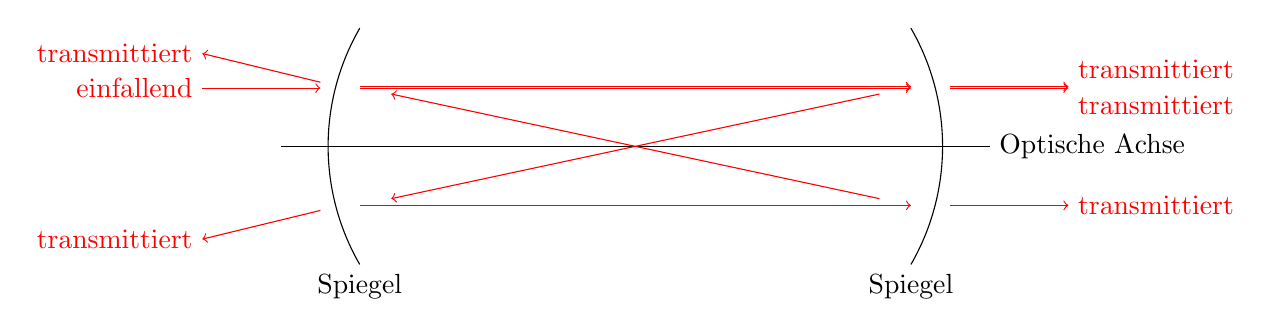
\begin{tikzpicture}
            \begin{scope}[yshift=+1.5cm]
              \draw (3,0) arc (150:210:3) node[anchor=north] {Spiegel};
              \draw (10,0) arc (30:-30:3) node[anchor=north] {Spiegel};
            \end{scope}
            \draw (2,0)--(11,0) node[anchor=west] {Optische Achse};
            \draw[color=red, <-] (2.5,0.74)--(1,0.74) node[anchor=east] {einfallend};
            \draw[color=red, ->] (3,0.74)--(10,0.74);
            \draw[color=red, ->] (10.5,0.74)--(12,0.74) node[anchor=south west] {transmittiert};
            \draw[color=red, ->] (9.6,0.75-0.4*1.5/7)--(3.4,-0.75+0.4*1.5/7);
            \draw[color=red, ->] (2.5,-0.75-0.3*1.5/7)--(1,-0.75-2*1.5/7) node[anchor=east] {transmittiert};
            \draw[color=red, ->] (3,-0.75)--(10,-0.75);
            \draw[color=red, ->] (10.5,-0.75)--(12,-0.75) node[anchor=west] {transmittiert};
            \draw[color=red, ->] (9.6,-0.75+0.4*1.5/7)--(3.4,0.75-0.4*1.5/7);
            \draw[color=red, ->] (2.5,0.75+0.3*1.5/7)--(1,0.75+2*1.5/7) node[anchor=east] {transmittiert};
            \draw[color=red, ->] (3,0.76)--(10,0.76);
            \draw[color=red, ->] (10.5,0.76)--(12,0.76) node[anchor=north west] {transmittiert};
          \end{tikzpicture}
          \caption{Aufbau eines \textit{Fabry-Perot-Etalons} aus zwei sph\"arischen Hohlspiegeln. Zus\"atzlich ist der Strahlengang eines einfallenden Lichtstrahls eingezeichnet. Nach $n\cdot 4$, $n\in\mathbb{N}$ Reflektionen setzt der Strahl seinen Weg hinter dem Interferometer geradlinig fort. Weitere Ausf\"uhrungen in \cref{subsec:fabry-perot-etalon}.}
          \label{fig:fabry-perot-etalon}
        \end{figure}


      \subsection{Linienbreite des verwendeten Diodenlasers}
      \label{subsec:linienbreite-laser}

        \begin{figure}[tb]
          \centering
           \begin{tikzpicture}
               \def\Vmin{-4}
               \def\Vmax{12}
               \def\tmin{-5}
               \def\tmax{5}
               %
               \begin{axis}[
                 /tikz/line join=bevel,
                 width=0.8*\textwidth,
                 height=0.5*\textwidth,
                 every axis plot,
                 grid,
                 legend style={at={(1,0.5)}, legend columns=1, anchor=north east},
                 axis y line*=left,
                 xmin = \tmin, xmax = \tmax,
                 ymin = \Vmin, ymax = \Vmax,
                 xlabel = {Zeit $t$ in $\si{\milli\second}$},
                 ylabel = {Spannung $V_\mathrm{ch2}$ in $\si{\milli\volt}$},
                 ]
                 % Add plots
                 \addplot[color = blue, only marks, mark options={scale=0.2}, line width = 1pt]
                 table [x=t, y=ch2]{data/linienbreite.txt};
                 \addlegendentry{ch2}
                 \addplot[color = red, line width = 1pt]
                 table [x=t, y=fit]{data/linienbreite.txt};
                 \addlegendentry{fit}
               \end{axis}
               \begin{axis}[
                 /tikz/line join=bevel,
                 width=0.8*\textwidth,
                 height=0.5*\textwidth,
                 axis y line*=right,
                 legend style={at={(1,0.5)}, legend columns=1, anchor=south east},
                 ymajorgrids=true,
                 xmin = \tmin, xmax = \tmax,
                 ymin = -50, ymax = 400,
                 ylabel = {Spannung $V_\mathrm{ch3}$ in $\si{\volt}$},
                 ytick = {-40, 0, 40}
                 ]
                 % Add plots
                 \addplot[color = green, only marks, mark options={scale=0.2}, line width = 1pt]
                 table [x=t, y=ch3]{data/linienbreite.txt};
                 \addlegendentry{ch3}
               \end{axis}
           \end{tikzpicture}
           \caption{Dopplerfreies Spektrum zur Bestimmung der Linienbreite des Diodenlasers. Die Spannung ch2 zeigt die Interferenzmaxima des \textit{Fabry-Perot-Etalons}. In rot ist ein f\"unffacher Gau\ss{}glockenfit zur Bestimmung der Halbwertsbreite der Maxima eingezeichnet. Zuletzt ist zeigt gr\"un den Verlauf der Spannungsmodulation des Netzteils zur Variation der Laserlichtfrequenz.}
           \label{fig:linienbreite-plot}
        \end{figure}

        Zur Bestimmung der Linienbreite wird der Laserstrahl direkt in das \textit{Fabry-Perot-Etalon} geleited und dahinter mit einer Diode als ch2 erfasst. Eine Dreiecksspannung ch3 varriert mithilfe eines Piezoelements währenddessen die Länge des Etalons. \Cref{fig:linienbreite-plot} zeigt die Messdaten des Laserspektrums. Hierbei liegen die ersten beiden Maxima von ch2 auf einem aufsteigenden Ast von ch3 und die zweiten beiden auf dem folgenden absteigenden Ast. Mithilfe eines mehrfachen Gau\ss{}fits werden die maxima genauer charakterisiert. Die Fitparameter sind in cref{subsec:fit-linienbreite} einzusehen.

        Der Abstand $\Delta t_\mathrm{FPE}$ zwischen den beiden Maxima der jeweiligen P\"archen entspricht gem\"a\ss{} \cref{subsec:fabry-perot-etalon} gerade dem \textit{freien Spektralbereich} des \textit{Fabry-Perot-Etalons} $Delta f_\mathrm{FPE}$ (vgl. \cref{eq:freier-spektralbereich}). Nun ist die \textit{Linienbreite} des Lasers gegeben durch den Zusammenhang
        \begin{equation}
          \Delta f_\mathrm{Laser} = \frac{\Delta f_\mathrm{FPE}}{\Delta t_\mathrm{FPE}}\cdot \Delta t_\mathrm{FWHM},
          \label{eq:deltaf-laser}
        \end{equation}
        mit der Halbwertsbreite der Maxima von ch2
        \begin{equation*}
          \Delta t_\mathrm{FWHM}=\frac{1}{2\sqrt{2\ln 2}\sigma}.
        \end{equation*}
        Hierbei ist $\sigma$ die Standardabweichung vom jeweiligen Gau\ss{}fit eines Maximums.

        Durch Einsetzen in \cref{eq:deltaf-laser} folgen die Werte
        \begin{align*}
          \Delta f_\mathrm{Laser}^\mathrm{aufsteigend, links}&\approx\SI{10,81(59)}{\mega\hertz} \\
          \Delta f_\mathrm{Laser}^\mathrm{aufsteigend, rechts}&\approx\SI{8,30(32)}{\mega\hertz} \\
          \Delta f_\mathrm{Laser}^\mathrm{absteigend, links}&\approx\SI{11,59(41)}{\mega\hertz} \\
          \Delta f_\mathrm{Laser}^\mathrm{absteigend, rechts}&\approx\SI{13,85(58)}{\mega\hertz}.
        \end{align*}
        Mitteln der zusammengeh\"orenden Werte liefert dann
        \begin{align*}
          \Delta f_\mathrm{Laser}^\mathrm{aufsteigend}&\approx\SI{9,56(34)}{\mega\hertz} \\
          \Delta f_\mathrm{Laser}^\mathrm{absteigend}&\approx\SI{12,72(36)}{\mega\hertz} ,
        \end{align*}
        und noch einmal mitteln f\"uhrt zu
        \begin{equation*}
          \Delta f_\mathrm{Laser}\approx\SI{11,14(25)}{\mega\hertz}.
        \end{equation*}

        \begin{table}
          \caption{Halbwertsbreite der Maxima von ch2, welche in \cref{fig:linienbreite-plot} abgebildet sind, sowie der Abstand der nach \cref{subsec:linienbreite-laser} zusammengehörenden Maxima. }
          \label{tbl:halbwertsbreite-daten}
          \selectfontsize{10pt}
          \begin{tabu} {X[r]X[r]X[r]X[r]X[r]X[r]}
            \unitoprule \\
            \multicolumn3{c}{\textbf{Aufsteigender Zweig}} &\multicolumn3{c}{\textbf{Absteigender Zweig}} \\\tabucline-
            $\Delta t_\mathrm{FWHM}^\mathrm{links}$ &$\Delta t_\mathrm{FWHM}^\mathrm{rechts}$ &$\Delta t_\mathrm{FPE}$  &$\Delta t_\mathrm{FWHM}^\mathrm{links}$ &$\Delta t_\mathrm{FWHM}^\mathrm{rechts}$ &$t_\mathrm{FPE}$ \\
            \tabuphantomline
            \unitoprule \\
            $-0,0396(20)$ &$0,0304(10)$ &$2,1958(16)$ &$0,0409(12)$ &$0,0489(18)$ &$2,1168(15)$ \\
            \unitoprule \\
          \end{tabu}
        \end{table}


      \section{Transmissionsspektroskopie}
      \label{sec:transmissionsspektroskopie}

        Zum Erstellen eines Termschemas von C\"asium werden Transmissionsspektren aufgenommen. Hierbei transmittiert der Laserstrahl durch die C\"asiumgaskammer und wird anschließend mit einer Diode erfasst. Erwartet werden Transmissionsminima an Stelle der Resonanzfrequenzen des C\"asiums, da hier Photonen die in \cref{fig:feinstruktur-hyperfeinstruktur} gezeigten \"Uberg\"ange der Atome anregen können und dabei absorbiert werden.


      \subsection{Dopplerverbreitertes Spektrum}
      \label{subsec:dopplerverbreitertes-spektrum}

        \Cref{fig:dopplerverbreitertes-spektrum} zeigt das dopplerverbreiterte Spektrum. Wie aufgrund der Dopplerverbreiterung (vgl. \cref{subsec:dopplerverbreiterung}) erwartet sind nur einzelne tiefe Minima im Spektrum zu sehen - nicht mehrere eng beieinander liegende Minima wie sie nach der Hyperfeinstrukturaufspaltung (vgl. \cref{sec:hyperfeinstruktur}) zu erwarten sind.
        Somit kann die Hyperfeinstruktur hier nicht untersucht werden. Im Folgenden soll die Feinstrukturaufspaltung vermessen werden. Dazu werden die beiden Minima vom Transmissionsspektrum ch1 betachtet, welche in \cref{fig:dopplerverbreitertes-spektrum} abgebildet sind. Diese befinden sich über einer einzelnen Rampe der Modulationsspannung des Netzteils.

        Das linke Minimum des Transmissionsspektrums geh\"ort zum Grundzustand $\mathrm{6^2S_{1/2}}$, das Rechte zum angeregten Zustand $\mathrm{6^2P_{3/2}}$. Für den Frequenzabstand zwischen Grundzustand und angeregtem Zustand$\Delta f_\mathrm{6^2S_{1/2}}^\mathrm{6^2P_{3/2}}$ gilt analog zu \cref{eq:deltaf-laser}
        \begin{equation*}
          \Delta f_\mathrm{6^2S_{1/2}}^\mathrm{6^2P_{3/2}} = \frac{\Delta f_\mathrm{FPE}}{\Delta t_\mathrm{FPE}}\cdot \Delta t_\mathrm{6^2S_{1/2}}^\mathrm{6^2P_{3/2}}.
        \end{equation*}
        \begin{equation*}
          \Delta t_\mathrm{6^2S_{1/2}}^\mathrm{6^2P_{3/2}}= \SI{6,9472(87)}{\milli\second}
        \end{equation*}
        ist hierbei der zeitliche Abstand zwischen den beiden angesprochenen Minima. Ein zweiundzwanzigfacher Gau\ss{}fit der Maxima von ch2 \"uber demselben Zweig von ch3 dient der Berechnung von
        \begin{equation*}
          Delta t_\mathrm{FPE}=\SI{0,4087(1)}{\milli\second}.
        \end{equation*}
        Dazu wurde der zeitliche Abstand zwischen dem ersten Auftretenden Maximum (1) und dem letzten (22) mithilfe der Fitparameter (\cref{subsec:fit-freier-spektralbereich-dopplerverbreitert}) durch $(22-1)$ Abstände geteilt.

        Somit ergibt sich der Frequenzabstand zu
        \begin{equation*}
          \Delta f_\mathrm{6^2S_{1/2}}^\mathrm{6^2P_{3/2}} = \SI{10,19(2)}{\giga\hertz}.
        \end{equation*}


        \begin{figure}[tb]
          \centering
          \begin{tikzpicture}
              \def\Vmin{0}
              \def\Vmax{12}
              \def\tmin{-4}
              \def\tmax{4.5}
              %
              \begin{axis}[
                /tikz/line join=bevel,
                width=0.8*\textwidth,
                height=0.5*\textwidth,
                every axis plot,
                grid,
                legend style={at={(0.5,0.5)}, legend columns=1, anchor=west},
                axis y line*=left,
                xmin = \tmin, xmax = \tmax,
                ymin = -60, ymax = 10,
                xlabel = {Zeit $t$ in $\si{\milli\second}$},
                ylabel = {Spannung $V_\mathrm{ch1}$ in $\si{\milli\volt}$},
                ytick = {-40,-30,-20,-10,0,10}
                ]
                % Add plots
                \addplot[color = red, line width = 1pt]
                table [x=t, y=ch1]{data/dopplerverbreiter.txt};
                \addlegendentry{ch1}
              \end{axis}
              \begin{axis}[
                /tikz/line join=bevel,
                width=0.8*\textwidth,
                height=0.5*\textwidth,
                axis y line*=right,
                legend style={at={(0.5,0.5)}, legend columns=1, anchor=east},
                ymajorgrids=true,
                xmin = \tmin, xmax = \tmax,
                ymin = 0, ymax = 50,
                ylabel = {Spannung $V_\mathrm{ch3}$ in $\si{\volt}$},
      					ytick = {0,5,15},
                ]
                % Add plots
                \addplot[color = blue, only marks, mark options={scale=0.1}, line width = 1pt]
                table [x=t, y=ch2]{data/dopplerverbreiter.txt};
                \addlegendentry{ch2}
                \addplot[color = blue!50, line width = 1pt]
                table [x=t, y=fitch2]{data/dopplerverbreiter.txt};
                \addlegendentry{ch2 fit}
              \end{axis}
          \end{tikzpicture}
          \caption{}
          \label{fig:dopplerverbreitertes-spektrum}
        \end{figure}


    \section{Dopplerfreie Spektroskopie}
    \label{sec:dopplerfreie-spektroskopie}


      \subsection{Cross-over Resonanzen}
      \label{subsec:cross-over-resonanzen}

        genau in der mittels


      \subsection{Dopplerfreies Spektrum}



        F\"ur die dopplerfreie Spektroskopie wird der Laserstrahl nun geteilt und antiparallel durch die Gaskammer geleitet. Derjenige Strahl, welcher analysiert wird (in diesem Fall mit dem \textit{Fabry-Perot-Etalon}), heißt \textit{Abfragestrahl}. Der andere ist der \textit{Anregestrahl}. Nun werden zwei Messungen durchgef\"uhrt. Einmal wird der \textit{Anregestrahl} geblockt, und einmal nicht. Im ersten Fall ensteht so ein dopplerverbreitertes Spektrum gem\"aß der Transmissionsspektroskopie. Im zweiten Fall aber regt der \textit{Anregestrahl} die C\"asiumatome in der Gaskammer an. Ist die Intensit\"at hinreichend hoch, so wird der Grundzustand entv\"olkert und der angeregte Zustand \"uberv\"olkert. Damit kann der \textit{Abfragestrahl} kaum noch Atome anregen und transmittiert fast ungehindert.


    \section{Zeeman-Effekt}
    \label{sec:zeeman-effekt}

      nicht observierbar!










\end{document}
